\documentclass[10pt]{article}

\usepackage{graphicx}
\usepackage{subcaption}
\usepackage{amsmath}
\usepackage{amsfonts}
\usepackage{fancyhdr}
\usepackage{minted}
\usepackage{comment}
%\usepackage{hyperref}
\usepackage{url}
%\usepackage{fancyvrb}

\setlength{\topmargin}{-.5in}
\setlength{\textheight}{9in}
\setlength{\oddsidemargin}{.125in}
\setlength{\textwidth}{6.25in}
\pagestyle{fancy}
\lhead{\footnotesize Timetagger Interface}
\rhead{\footnotesize Kwiat Quantum Information Group}
\definecolor{bg}{rgb}{0.95,0.95,0.95}
\begin{document}
\title{Timetagger Interface}
\author{Daniel Kumor}
\date{\today}
%\date{}
\maketitle
\abstract{Special software for time-to-digital converters allows for streaming time tags into a buffer at rates of over 50M$\frac{counts}{second}$.
The buffer is constructed in a way which allows for analysis of streaming data by multiple independent applications.
Programs for interfacing with 3 different TDC versions are described, and several commonly used analysis functions are provided.}
\tableofcontents
\clearpage
\section{Introduction}
Time tagging units can mimic the functionality of several hardware devices, such as singles and coincidence counters.
The time tags gathered by such units can also greatly simplify several tasks which are usually done manually, such as
finding delays between pulses. The data they gather can further be used for more difficult tasks, such as finding delays
between two noisy signals, or finding coincidences between multiple channels which usually require several AND, OR or NOT gates.
With the correct software, a time tagger can be made into a powerful tool for research. This document describes an attempt at
creating such software.

The document is divided into 3 main parts. First, software made to interface with different models of TDC is described from a user's standpoint. Next, the main program library which enables portably connecting interface software to analysis code is
described from a programmer's standpoint. Lastly, several extra methods for interfacing with the main program library and analysis
code are shown.

\section{Time Taggers}
\subsection{UQD-Logic-16}

\begin{figure}
\centering
\begin{subfigure}[b]{0.4\textwidth}
\includegraphics[width=200px,angle=-90]{UQD1.jpg}
\end{subfigure}
\qquad
\begin{subfigure}[b]{0.4\textwidth}
\includegraphics[width=200px,angle=-90]{UQD2.jpg}
\end{subfigure}
\caption{The UQD-Logic-16 time tagger}
\label{fig:uqd_pic}
\end{figure}

The Universal Quantum Devices time tagger (shown in figure \ref{fig:uqd_pic}) has a bin 
resolution specified at $156.25$ picoseconds, and can stream tags at rates up to $7$ MHz.
The time tagger requires a NIM crate with functional 5V and 12V outputs.
\subsubsection{Installation}
Refer to time tagger media for installation instructions. 
You will need to install the time tagger USB driver. In Kwiat lab, the lab file server contains all necessary driver files
with the time tagger's interface program.
For the software, you will also need the VC++ 2010 redistributable, and the .NET frameworks 2.0 and 4.0.
Most windows computers have these installed by default\footnote{If they are not installed on your computer, then
google should show you how to install them in no time.}
\subsubsection{Software}
The software is a $C\#$ program called ``TimeTagger.exe". Upon running, you should be presented with the
following window:

\begin{center}
\includegraphics{uqd_setup.png}
\end{center}

If you are just starting out, the defaults should work, so click Start. If you feel like experimenting,
the buffer size is the amount of data points to keep in memory (At least 50 million is recommended), and
the Time Tagger Number is the number of time tagger to open. Usually this is 1, but you could have multiple
time taggers connected to the same computer - in which case you can use trial and error to
find the correct number.

\begin{center}
\includegraphics{uqd_main.png}
\end{center}

The next screen is the ``business" end of the software. To start taking data, click ``Runner +". At this point
the buffer is filling with time tags, and can be accessed from the Matlab functions or any other libTTag interface.

The simplest way to save data is to click on the file icon in the bottom right hand corner of the software. This
will allow you to write a file with the data points currently in the buffer.

A console version of the software is also available. This version has the same interface as the Agilent and quTau
time taggers, with a configuration file ``uqd.uqcfg". Refer to the Agilent and quTau sections of this
document for details on usage.

One thing to note: The console version does not include a linux makefile. It can be compiled by
putting buffer.c and ttag.h from libttag/src as well as uqd.cpp into the directory where CppDemo.cpp is located
(CppDemo.cpp comes with the time tagger's software), and 
adding the following to the makefile\footnote{If compiling in this way, you will also need to change CTimeTag.h to be included in the same way as in CppDemo.cpp.}: 

\begin{minted}[mathescape,bgcolor=bg]{bash}
g++ -m64 buffer.c uqd.cpp -oUQDinterface -lpthread -lstdc++ -ICTimeTagLib 
	-L../CTimeTag/Linux -lusb-1.0 -ltimetag64 -lm -lrt 
	-lboost_program_options -lboost_thread 
\end{minted}

\subsubsection{Troubleshooting}
\paragraph{Time tagger gives errors when given 10 MHz reference}
The 10 MHz reference requires $50\ \Omega$ termination when using a logic signal. The time tagger gives errors if
that is not in place. Channel 16 cannot be used while reference is in place.

\paragraph{The time tagger streams bogus data despite not being connected to anything:}

We found the device to be extremely sensitive to voltage fluctuations. While using the device we quickly
found which NIM crates were not stable enough. Trying in another NIM crate might be a good bet. If
that is not an option, restarting
both interface software and time tagger should temporarily put the device into working order.

\paragraph{Software gives system error, "operation not supported by device", or other hardware error:}

You probably didn't install the driver software! The UQD time tagger needs a ``WinUsb" driver. To install it on Windows,
you will need to go to device manager, where there will be an unrecognized device. Right click, and select install/update
driver. Afterwards, choose to search for driver software on computer, and navigate to the folder containing all driver files.
The time tagger should then be recognized, and the software should start working.


\paragraph{USB Driver Issues:}


Older time tagger firmware versions had an issue interfacing with the computer when other devices were connected to USB ports
on the same computer. 
These issues are evidenced by:
\begin{enumerate}
\item ``Pipe error" in software;
\item ``Could not open device" in software;
\item Problems using time tagger with other USB devices;
\item Computer not booting with usb devices plugged in after driver installation.
\end{enumerate}
This is a problem with the device driver/firmware. Make sure you have the most recent firmware and driver software.
If all else fails, try to make sure the time tagger is plugged into its own dedicated USB port, and not into a hub. 
Dedicated ports are usually the ones directly on the motherboard. Also, we found that in some cases, unplugging all
USB devices other than the time tagger can help\footnote{Computer has to be accessed through remote desktop software in this case,
since }. This problem is fixed in firmware as of 11/15/2013.


\subsection{Agilent Acqiris U1051A}
\begin{figure}
\centering
\begin{subfigure}[b]{0.4\textwidth}
\includegraphics[width=200px,angle=180]{Agilent1.jpg}
\end{subfigure}
\qquad
\begin{subfigure}[b]{0.4\textwidth}
\includegraphics[width=200px,angle=180]{Agilent2.jpg}
\end{subfigure}
\caption{The Agilent TC890 time tagger}
\label{fig:agilent_pic}
\end{figure}

The Agilent Acquiris TC890 (U1051A) time tagger shown in figure \ref{fig:agilent_pic} has a bin resolution specified at 50 picoseconds,
and we have found it can stream tags at rates of over 25 MHz. It also has several features such as a veto input,
trigger channel, and a 10 MHz reference input which make this a very powerful piece of hardware.
It also requires a careful setup, and we found that returned data is sometimes unordered, especially when running
at higher rates. Software was made to account for these problems.

\subsubsection{Installation}

\textbf{WARNING: Make sure the data is backed up on any computer on which you attempt installing the Agilent. We had some problems associated with the stability of certain systems when this timetagger's PCI card and drivers were installed.}

To start off, the Agilent time tagger comes with a PCI card. Many PCI slots do not work properly with this
hardware\footnote{Finding a working computer/PCI slot seemed to be a matter of trial and error. 
We tried it in several different computers, and found that only one model worked. Furthermore, our collaborators had
the same model of computer (Dell T7500), with the same software and BIOS versions - and the card worked in different slots.}.
For each slot you try, you should install the driver software, and see if the computer crashes/freezes when the time tagger is
plugged in.

One important thing to note is that the hardware is connected to a computer using PCI extension, meaning that the timetagger
must be plugged in and turned on before the computer is powered on. Furthermore, the timetagger must not be disconnected
from the computer while the computer is turned on. Turning the TDC off while the computer is on can lead to some nasty
consequences\footnote{Such as a blue screen of death. We also experienced system corruption, but are not sure whether the 
Agilent caused this specific error.}.
\subsubsection{Software}

The software is a 64 bit C++ program called ``Agilent.exe". Running it should pop up a console window as such:
\begin{center}
\includegraphics[width=\textwidth]{agilentconsole.png}
\end{center}
The console program is non-interactive. All interaction is through the buffer (the figure shows buffer 0 in this case).

Timetagger settings are put into a configuration file ``ttAgilent.agcfg".
In the configuration file, the threshold voltages for each channel can be set, and veto/10MHz reference can be enabled.
The configuration file is located in the same folder as the executable. The file should be fairly well documented by default,
but to see a list of available properties, you can open the command line to the folder containing ``Agilent.exe", and
run ``Agilent.exe --help", which will display a list of all available commands that the program accepts.

\subsubsection{Troubleshooting}
\paragraph{I get double pulsing/lost tags:} The time tagger has fuses which automatically trigger on signals over 5V,
which might cause lost tags if the signal has too large of a voltage. We found that frequently double pulsing was related to
the connections that our cables had with the time tagger. We never really figured out a method other than trial and error
for fixing this issue.
\paragraph{Error initializing/calibrating:} This error is most frequently encountered when the 10 MHz reference
is enabled, but the time tagger does not have an active 10MHz input connected. Setting ``reference=0" in the configuration
file should set you right in no time.
\paragraph{ERROR: Tag out of bounds! (Check firmware version!):} If you get this error,
it means that a time stamp was detected which was larger than the maximum stamp that the time tagger allows. This
happens between switches in the time tagger's internal buffer on older firmware versions. The newer version of firmware
no longer shows this problem.
\paragraph{The timetagger is not found/unrecognized:} If the driver software is installed, then sometimes restarting the
computer and time tagger helps. If this fails to resolve the problem, then changing PCI slots for the interface card
might help. Or it might not.
\paragraph{I have two of these time taggers. I can't get the second one to initialize!} For some reason we were unable to
get the Agilent software to run simultaneously from different processes. We worked around this problem by creating a special
program which opens all available Agilent time taggers simultaneously. The downside is that all connected time taggers
will be initialized to the same settings.

\subsection{Qutools quTAU}
The qutools quTau time tagger has a bin resolution of 81ps. We have found that it can stream tags at rates of over 
6 MHz\footnote{The rate we found is over double the specification of 3 MHz continuous count rate.}. This time tagger has 8 inputs,
which are triggered on TTL signals. The threshold levels are not adjustable, and it does not have a 10 MHz 
reference\footnote{The lack of a reference input disallows the straightforward synchronization of the hardware 
clocks of multiple TDCs. There
are ways around this, such as dedicating a channel to ``clock" input, and doing manual synchronization.}.

\subsubsection{Installation}
The drivers for this time tagger are available at the qutools website after purchase of the quTau time tagger. 
Our software for this hardware was only compiled for 64 bit windows computers, although there should be 
no difficulty compiling it on 32 bit platforms or on linux if necessary. The MSVC 2010 redistributable is needed for the
software


\subsubsection{Software}

The software is similar in form to the Agilent executable. Here, we have ``quTAU.exe", with configuration file ``qutau.qucfg".
The C++ setup and configuration code is shared with both the Agilent and console version of the UQD time tagger software.
This means that ``quTAU.exe --help" in a console should list all available commands. Again, the default configuration file
should be fairly well documented.

%\subsubsection{Troubleshooting}


\section{Timetagger Library}
\subsection{General Idea}
Originally, when wanting to do work with time taggers, our procedure was as follows:
\begin{enumerate}
\item Run time tagger, saving tags to RAM;
\item After taking data, write contents of RAM to file;
\item Open file in Matlab, and run analysis routines on resulting arrays.
\end{enumerate}

This was not optimal: the intermediate step of writing a file was wasteful for our purposes.
To make the process as simple as possible, it would be best if analysis could be performed on the tags as they come in.
Furthermore, it would be useful if many unrelated programs could access the time tags at the same time. In our case, quantum
cryptography code could be tested on the data at the same time as Matlab programs would display live plots of efficiencies for
optical adjustments. Lastly, we had
several different time taggers, all of which had different methods of interfacing with code - making all of them work with minimal
changes to the programs' logic would be a fantastic bonus. To that end, the following requirements were created for the time tagger library:

\begin{itemize}
  \item Must be able to get time-stamps in real-time
  \item Time tags should be accessible to many different applications at the same time
  \item Changing physical time taggers should not require rewrites of analysis/user code
  \item Time tags should be accepted much faster than a file can be written ($>1$ GB/s)
  \item Basic time tag processing/analysis code needs to be provided with the library.\footnote{Telling grad students that they don't have to write their own analysis code puts a smile on their face}
\end{itemize}

\begin{figure}
\begin{center}
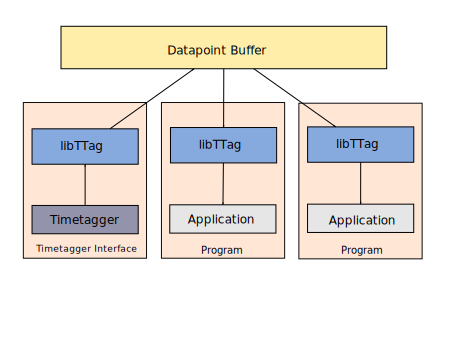
\includegraphics[width=250px]{libttag.png}
\caption{The timetagger library creates a datapoint buffer in memory, which is independent of the programs accessing it, allowing multiple programs to read and write to it at the same time.}
\label{fig:libttag}
\end{center}
\end{figure}

These goals were achieved by using named memory maps, in effect making a piece of memory available to many programs at the same time (fig \ref{fig:libttag}). The library takes care
of synchronization and abstracts away the details of reading and writing time tags. While the functionality
is written in C, most languages provide methods of using native libraries in their code.

For timetag processing, multiple functions were created to find statistics regarding the data, such as singles/coincidence counts and correlations between channels.

The library does have one limitation, which has to do with the amount of free memory available. The `buffer' cannot
keep more data points than there is RAM. Once the memory is full, libTTag will overwrite the oldest data
with new data points by default. If one requires all data to be present, it is important to make the buffer
large enough to contain it, or to write to a file during acquistion!

%Note: To have API show up in the table of contents, the footnote needs to be removed, the program compiled, and then the footnote
%   put back in
\subsection{Functionality}
This section is to explain the library's specifics - how to interface with libTTag, and the details of 
algorithms used for data analysis functions. 

\subsubsection{Buffer}
The buffer is the core of the library - it provides functions which do manipulation and synchronization necessary to abstract away details of shared memory. This section will not list or explain the library's inner workings\footnote{I don't have the patience
to do that! If you want to see the details of memory mapping, the code should be fairly well documented.}. Rather, this attempts to give a very basic review
of the most important things implemented - the stuff that one needs to know to use libTTag. For a complete reference,
open the library's main header file (ttag.h), which contains documentation for all available functions.



\paragraph{Opening and closing the buffer:}
To start off, you need to create the buffer. This amounts to registering memory such that it is available to other programs. The following code creates a buffer:

\begin{minted}[mathescape,bgcolor=bg]{c}
int buffernum = tt_getNextFree();\

//libTTag provides the tt_buf structure, which holds connection to data.
tt_buf* mybuffer = tt_create(buffernum,50000000);

//Make sure that the buffer was created
if (mybuffer) {
    printf("Buffer number: %i",buffernum);
} else {
    printf("Failed to create buffer");
}
\end{minted}

The key function in the given code snippet is tt\_create:

\begin{minted}{c}
tt_buf* tt_create(int mapnumber,uint64_t datapoints);
\end{minted}

Like the name suggests, this function creates a new buffer for a time tagger. It has two inputs:

The first is the `buffer number' to create; the buffer number is a number identifying the time tagger, since multiple time taggers could be using libTTag at the same time! Starting from 0 is a good bet if testing, but I recommend
using tt\_getNextFree to find an available number (as shown in the sample).

The second term is the number of data points that the buffer should be able to hold
at one time\footnote{Please note that on Linux, the number of data points that can be held is limited by the allowed size
of shared memory. It is possible to force Linux to allow almost the entire RAM to be used by changing 
certain settings.}. I suggest making this a very large number (at least 1 million). A buffer that can hold 50 million data points
takes less than 500 MB of memory.

Suppose now that the buffer was already created with tt\_create. It so happened that
buffer number 0 (the first available buffer) was chosen. To open it from another application, tt\_open is used:

\begin{minted}[mathescape,bgcolor=bg]{c}

tt_buf* mybuffer = tt_open(0);

//Make sure that the buffer was opened
if (mybuffer) {
    printf("Buffer open!");
} else {
    printf("Failed to open buffer. Did you create one first?");
}
\end{minted}

The function is defined as:

\begin{minted}{c}
tt_buf* tt_open(int mapnumber);
\end{minted}

After these two commands, the creating program and the opening program both have access to the exact
same location in RAM, meaning that data put into the buffer is immediately available to the other program.

When finished, the buffer must be closed so that its memory is deallocated\footnote{On Linux, the buffer is destroyed when tt\_close is called from the program which ran tt\_create, while on Windows, it is
destroyed once there are no programs using it. This means that timetagger interface code should not close
the buffer until it is not needed!}. This is done with:

\begin{minted}{c}
void tt_close(tt_buf* buffer);
\end{minted}

An example of both creation and destruction of a buffer is:

\begin{minted}[mathescape,bgcolor=bg]{c}
int buffernum = tt_getNextFree();
tt_buf* mybuffer = tt_create(buffernum,50000000);

//Do stuff

tt_close(mybuffer);

\end{minted}

\begin{figure}
\begin{center}
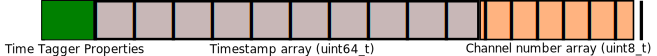
\includegraphics[width=350px]{bufferstructure.png}
\caption{The buffer's memory consists of three main parts: 1) Storage for the time tagger's properties such
as resolution and channel count; 2) array for storing time stamps; and 3) array for storing channel numbers
corresponding to the timestamps.}
\label{fig:bufferstructure}
\end{center}
\end{figure}

\paragraph{Reading and writing timetags:} Once the buffer is open, everything is ready to start taking data!
Two internal arrays are used to store time tags. The first array is to store the time stamp of the data point, while the second is to store the tag's channel\footnote{Channel data is stored in an array of type uint8\_t, meaning that libTTag can store data for up
to 256 channels. Time tags are stored as unsigned 64 bit integers, so even if the time tagger
were to have a resolution of 1 picosecond, it would take over half of a year of continuous data-taking 
to overflow the counter. Of course, the amount of data that can actually be stored at one time is limited by RAM.}
(Figure \ref{fig:bufferstructure})
.

LibTTag makes one major assumption about the time tags, which is not always true
of data that comes right from a time tagger. LibTTag requires time tags to be increasing;
the analysis and search functions explicitly assume that the tags are ordered. This requirement is the
greatest difficulty of interfacing a new time tagger with libTTag. 
While most time taggers return ordered tags, some have internal
counters that might overflow, meaning that there are moments when a new time tag has a smaller time stamp
than an earlier one from the same channel. LibTTag does not handle these overflows by itself. It is the
job of the time tagger's interface code to provide methods for detecting overflows and correcting them.
An example of a way to do this is provided in the samples. The requirement that tags be ordered makes
the users' lives much easier - and makes it simpler to write analysis code that is independent of time tagger
idiosyncrasies.

That being said, there exist several methods for accessing the buffer\footnote{For all of the following code $mybuffer$ is assumed to be initialized by libTTag as shown earlier.}. Suppose you have a new datapoint, and
want to add it to the end of a buffer:

\begin{minted}[mathescape,bgcolor=bg]{c}
uint8_t  channelnumber = ...
uint64_t timestamp     = ...

tt_add(mybuffer,channelnumber,timestamp);
\end{minted}

The add function used above is defined as:

\begin{minted}{c}
void tt_add(tt_buf *buffer, uint8_t channel, uint64_t timetag);
\end{minted}

The method for reading the most recent data point into your variables is similar:

\begin{minted}[mathescape,bgcolor=bg]{c}
uint8_t  channelnumber = 0
uint64_t timestamp     = 0

tt_read(mybuffer,0,&channelnumber,&timestamp);

//The most recent datapoint is now written to the two variables
\end{minted}

One may now wonder why the extra 0 argument in the add function. This is because we wanted to read the most
recent data point, which is 0th from the most recent element! For example, reading the nth most recent
data point can be achieved by:

\begin{minted}[mathescape,bgcolor=bg]{c}
tt_read(mybuffer,n-1,&channelnumber,&timestamp);
\end{minted}

These functions are the simplest methods of accessing the buffer.
They are also the least practical
when doing major interfacing/analysis work, since one rarely reads/writes 
points one at a time\footnote{Not to even mention that they are the slowest.}.

The most useful access functions deal in arrays. Reading and writing by arrays is fast, efficient,
and infinitely more useful than doing so element by element:

\begin{minted}{c}
void tt_addarray(tt_buf *buffer, uint8_t *channels, uint64_t *timetags,
                uint64_t datapoints);
uint64_t tt_readarray(tt_buf *buffer,uint64_t startpoint, 
                uint8_t *channel, uint64_t *timetag, uint64_t datapoints);
\end{minted}

The only difference from $tt\_read$ to $tt\_readarray$ is the additional argument stating the number of data points
to write. In fact, $tt\_read$ is just a macro using $tt\_readarray$ with $datapoints=1$.

There are two differences between $tt\_add$ and its array counterpart. First off, like in read, there is
the added number of data points to write. The next difference is that it accepts arrays rather than
single data points, for obvious reasons.

\begin{minted}[mathescape,bgcolor=bg]{c}
//Time tags to write
uint8_t  channelnumbers[10000] = ...
uint64_t timestamps[10000]     = ...

//Time tags to read
uint8_t read_channels[100];
uint64_t read_timestamps[100];

//Add the 10000 time tags to the end of the buffer
tt_addarray(mybuffer,channelnumbers,timestamps,10000);

//Read the most recent 100 data points to the two read arrays
tt_readarray(mybuffer,0,read_channels,read_timestamps,100);
\end{minted}

These array functions are the recommended way to access the time tagger.

Next, you might want to read data straight from the buffer without using intermediate arrays 
to conveniently implement an analysis routine.
In that case, libTTag also provides direct access to the internal memory through C macros:

\begin{minted}{c}
#define tt_writeindex(buffer)         ...
#define tt_channel(buffer,datapoint)  ...
#define tt_tag(buffer,datapoint)      ...
#define tt_datanum(buffer)            ...
\end{minted}

These macros can be used in mostly
the same way as an array\footnote{You can't do memcpy from/to them, since the next element is not 
guaranteed to be the next location in memory.}, meaning that one can read and write tags right
into them:

\begin{minted}[mathescape,bgcolor=bg]{c}

uint64_t tags[500] = ...
uint8_t channel[500] = ...

//Adding 500 datapoints to the buffer
tt_writeindex(mybuffer) += 500;
for (int i=0; i< 500;i++) {
    tt_channel(mybuffer,tt_datanum(mybuffer))=channel[i];
    tt_tag(mybuffer,tt_datanum(mybuffer))=tags[i];
    tt_datanum(mybuffer)++
}

//Read most recent datapoint
uint8_t channel = tt_channel(mybuffer,tt_datanum(mybuffer)-1);
uint64_t timetag = tt_tag(mybuffer, tt_datanum(mybuffer)-1);


\end{minted}

tt\_datanum gives the number of time tags that the buffer handled. To put simply, it returns
the total number of time tags that the buffer would have if it had infinite memory, ie, no overflow.

tt\_channel gives direct access to the channel array, and tt\_tag gives access to the tag array.

People used to Matlab should remember that
the arrays start from index 0, meaning that the `next free' element is of index $tt\_datanum$ and
the `most recent data point' has index $tt\_datanum-1$.

Three things to note: 
\begin{enumerate}
\item The array index here is the opposite of the earlier access methods, where the index meant
number from the most recent point. Here, it means ``I want the nth data point that libTTag registered".

\item When using these macros, one does not have to worry about tt\_datanum becoming larger than the buffer.
They contain code which makes sure that tags are put in the right spot. 

\item When writing tags using the macros, tt\_writeindex should be first, and tt\_datanum++ needs to be the last command, such that other
programs don't try to access the newest tag while it is being written!

\end{enumerate}

I have personally found these macros to be my preferred method of buffer access. 

Lastly, sometimes even this won't do - the timetagger might just be streaming data too fast
for constant memory allocations or validity checks. In that case, you will need to go straight for the internal memory arrays.
To see how this is done, look at the source code for $tt\_writearray$. With a good computer, libTTag is able to write over 300 million time stamps a second
when using the internal memory. It is not recommended that you try this unless you are confident that you understand the assumptions 
libTTag makes regarding its internal buffer arrays, and really, truly need the speed.


\subsubsection{Tag Analysis}
Functions for getting information about the data stream are located in analysis.c. There are 5 main function types available:
\begin{enumerate}
\item Singles counting - can give the number of time tags (counts) overall in each channel within a given time period.
\item Coincidence counting - gives a matrix of coincidences of each channel to each channel within a given time period.
\item Team coincidences - given an array of channels (not necessarily all different), returns the number of times that at least one unique pulse from all the channels was
detected within the given time period.
\item Correlation - allows to do a cross-correlation of two arbitrary channels in the buffer given a bin size and time period.
%\item Delay - can find delays between channels with noisy data if they are less than the pulse rate for the channels (useful for finding delays due to small experimental imperfections)
\end{enumerate}

\paragraph{Finding singles counts} Getting counts is done using the function 

\begin{minted}{c}
uint64_t tt_singles(tt_buf* buffer, double time, uint64_t* channelSingles);
\end{minted}

Like everywhere else in libTTag, the first argument is the buffer object. The second argument is a time period in seconds for which singles
should be counted. The function reads data starting from the most recent time stamp, ie the current time. ``Current time" is dependent on the time tagger interface.
Some time taggers will only update the reference time once in a short interval if not recieving time tags, meaning that if there is no data coming in,
the results of $tt\_singles$ might not be exact. The last argument is optional, an array into which per-channel singles are put.

Basic usage is as follows:

\begin{minted}[mathescape,bgcolor=bg]{c}

uint64_t total_singles = tt_singles(mybuffer,0.5,NULL);
printf("Total number of tags in the last half second: %i\n",(int)total_singles);

\end{minted}

If you want to get the singles count for each individual channel, you can input an array of channel size, and per-channel singles will be returned:

\begin{minted}[mathescape,bgcolor=bg]{c}
uint64_t total_singles;
uint64_t *channel_singles;
int i;

//Allocate array of zeros to hold singles for each channel
channel_singles = calloc(sizeof(uint64_t),tt_channels(mybuffer));

total_singles = tt_singles(mybuffer,0.5,channel_singles);

printf("Total number of tags in the last half second: %i\n",(int)total_singles);

for (i=0;i<tt_channels(mybuffer);i++) {
    printf("Channel %i: %i\n",i,(int)channel_singles[i]);
}

free(channel_singles);
\end{minted}

There is also a $tt\_rawsingles$ available, which is used by $tt\_singles$ internally. It allows more fine-grained control. Refer to the main header file for further documentation.

\paragraph{Getting coincidences} Finding the number of pulses that are in coincidence between two channels is done using:

\begin{minted}{c}
uint64_t* tt_coincidences(tt_buf* buffer, double time, double radius, \
                    uint64_t* coincidenceMatrix, double* delayArray);
\end{minted}

The ``time" is time in seconds (starting from now, the reference time, and going backwards) to search for coincidences. The coincidenceMatrix parameter allows you to allocate your own array for the matrix of coincidence (explained later). If unclear on how to use, just set it to NULL, and the function will allocate the matrix for you. If you let the function allocate the matrix, it will need to be ``freed" using $tt\_free$!

\begin{figure}
\begin{center}
\includegraphics[width=250px]{diameter.png}
\caption{In order to find coincidences between channel 1 and 2, it is necessary to define a time period around a pulse of channel 1 within which a pulse of channel 2 is considered a coincidence.}
\label{fig:diameter}
\end{center}
\end{figure}

\textbf{Radius of Coincidence:} When trying to find coincidences (pulses that are correlated between two channels), it is necessary to define what time period is counted as
valid. With fast TDCs, even identical function generator pulses are sometimes registered at slightly offset times. The radius of coincidence is half of the diameter of coincidence,
shown in figure \ref{fig:diameter}. It is counted in seconds.

\begin{figure}
\begin{center}
\includegraphics[width=250px]{delays.png}
\caption{Pulses between channels might be correlated but offset by a certain constant time period. Setting a delay accounts for this.}
\label{fig:delays}
\end{center}
\end{figure}

\textbf{Delays:} Often, one signal has to travel a different path than its correlated counterpart. This means that even if the two channels (signals) are correlated, 
their time stamps might be offset by a constant delay (figure \ref{fig:delays}).
When a function has as one of its parameters ``delays between channels", it can take such offsets into account. Delays are given in seconds. 
In most cases the delay between channels can be found using $tt\_delay$.

$tt\_coincidences$ outputs an array of size $channels*channels$, which is a flattened matrix of the number of coincidences detected between each two channels. For example,
if you want to find the number of coincidences in the last second between channel 0 and 5, you can do the following:

\begin{minted}[mathescape,bgcolor=bg]{c}
uint64_t *coincidenceMatrix;

coincidenceMatrix = tt_coincidences(mybuffer,1.0,1e-5,NULL,NULL);

if (coincidenceMatrix) {
    //Singles of each channel are stored in the diagonal elements of the matrix.
    //Notice the coincidenceMatrix is flattened into an array.
    printf("Channel 0 singles: %i\n", (int)coincidenceMatrix[tt_channels(mybuffer)*0+0]);
    printf("Channel 5 singles: %i\n", (int)coincidenceMatrix[tt_channels(mybuffer)*5+5]);

    //The matrix is symmetric, so it doesn't matter which channel comes first
    printf("Coincidences between channels 5 and 0: %i\n", \
                (int)coincidenceMatrix[tt_channels(mybuffer)*5+0]);

    tt_free(coincidenceMatrix);
}
\end{minted}

\paragraph{Team Coincidences} Coincidences between more than two channels at once are found using the following:

\begin{minted}{c}
uint64_t tt_multicoincidences(tt_buf* buffer, double time, double diameter, \
            uint8_t* channels, int channelnum, double* delayArray);
\end{minted}

\begin{figure}
\begin{center}
\includegraphics[width=250px]{multicoincidence.png}
\caption{A ``team coincidence" (multi-coincidence) is registered when all relevant channels have at least one pulse within the given diameter.}
\label{fig:multicoincidence}
\end{center}
\end{figure}

The first two arguments are the buffer object (explained multiple times already), and time, the number of seconds of data to use in calculations.
The third argument, diameter, is the distance within which at least one pulse of each channel is located (Figure \ref{fig:multicoincidence}). After
that comes an array of channels you want to test for coincidences, and the size of this array. There is also an optional array of delays, which is explained
in the previous section on $tt\_coincidences$. Note that here, the array of delays refers to the delays for the channels passed in, and not all channels
in the buffer, as with $tt\_coincidences$. Usage example:

\begin{minted}[mathescape,bgcolor=bg]{c}
//Create an array for the channels you want to check
uint8_t channels[4] = {0,1,3,5};

//Find coincidences
uint64_t coincidences = tt_multicoincidences(mybuffer,1.0,1e-4,channels,4,NULL);

printf("Coincidences between channels 0,1,3 and 5: %i\n", (int)coincidences);

\end{minted}

\paragraph{Correlations between channels}
An implementation of windowed cross-correlation. For an explanation of what it is: \url{http://en.wikipedia.org/wiki/Cross-correlation}.

\begin{minted}{c}
uint64_t* tt_correlate(tt_buf *buffer, double time, double windowradius,\
                        int bins, uint8_t channel1, double delay1, uint8_t channel2,\
                        double delay2,uint64_t* resultArray);
\end{minted}

The first two arguments, the buffer object and the time, are the same as everywhere else. The time is the number of seconds of data
to include in the calculation. Next comes the windowradius and bins. 

\begin{figure}
\begin{center}
\includegraphics[width=250px]{correlation.png}
\caption{A correlation can be done knowing the diameter of window for each pulse of channel 1, and a number of bins into which to subdivide the window. Note that the function tt\_correlate uses
a window radius, which is $\frac{1}{2}$ the diameter.}
\label{fig:correlation}
\end{center}
\end{figure}

The two terms are explained in figure \ref{fig:correlation}. For each pulse of the first channel, a window of the given radius is created, and subdivided into the given number of bins (the amount of bars that would show up on a histogram).
From that, the cross-correlation between the two channels can be found.
The next 4 arguments are the 2 channels to correlate, and their associated delays. The delays are the same thing as described in figure \ref{fig:delays}.
Lastly, the resultArray is an optional array of size ``bins" into which to put the answers. If you put in NULL, an array will be allocated, and will need to
be freed using tt\_free. Here's a usage sample:

\begin{minted}[mathescape,bgcolor=bg]{c}
int bins =500;  //We want 500 bins

//Find cross-correlation with a window diameter of 0.01s (0.005s radius)
//  of 1 second of data, btwn channels 2 and 5 (with 0 delays)
uint64_t* correlation = tt_correlate(mybuffer,1.0,0.005,bins,2,0.0,5,0.0,NULL);

if (correlation) {
    for (int i=0; i < bins; i++) {
        printf("%i\t%i\n",i,(int)correlation[i]);
    }
    tt_free(correlation);
}
\end{minted}

%\paragraph{Finding delays between channels}


\subsection{Examples}
\subsubsection{Template for interfacing TDC}

\inputminted[mathescape,bgcolor=bg]{c}{Examples/interfacing_timetagger.c}

\subsubsection{Template for analysis of time stamps}

\inputminted[mathescape,bgcolor=bg]{c}{Examples/using_timetags.c}

\subsection{Compiling}
\subsubsection{Windows}
You will need Microsoft's Visual Studio with its C++ compiler. There is a MSVC directory in the libTTag folder. This folder contains a prepared 
Visual Studio project file, which is configured and ready. From there, it is a matter of making sure that the build configuration is set to ``Release",
and clicking the ``play" button (or going through menus, and running a build). There should pop up a test window. If all tests pass, libTTag works on your system.

At this point, you can either just include libTTag's source files in your own projects (easiest\footnote{In order for the code to compile, 
you need to set it to use the multibyte character set, rather than unicode. This should be in the general C/C++ settings. For the analysis code to work, you also need
to force MSVC to use the C++ compiler on the C code, since MSVC's C compiler sucks 
(this option should be in Configuration Properties / C/C++ / Compile As / Compile As C++ Code (/TP)).}), or you can use the libTTag DLL and .lib file you just created.
The files are located in the MSVC/libTTag/Release/ directory. You will need both libTTag.dll and libTTag.lib. I am assuming that if you choose this route, you
know how to go from there.


\subsubsection{Linux}
Make sure that you have a C/C++ compiler as well as $make$ installed. The first thing to do is make sure that the code works on your computer!
Go to the libttag/test directory and open a terminal there. Type in ``make". After several seconds and multiple possible warnings about char* conversions,
there should appear a file called ``$libttag\_test$" in the directory. In the same terminal, type in ``$./libttag\_test$", which will run tests of libTTag's 
functionality. If all tests pass, it means that libTTag seems to work correctly on your system!

Once that is done, libttag.a should exist in the libttag directory, ready to be used.

The following sequence of commands in the $libttag$ directory summarizes the previous paragraph:

\begin{minted}[mathescape,bgcolor=bg]{bash}
cd ./test
make
./libttag_test
cd ..
\end{minted}

By default, g++ is used as the compiler. Clang has been shown to work also. One thing to note is that when creating a ``.a" file, you must use the same compiler
as your final project. For example, creating the .a file with gcc and then attempting to use it with g++ might fail. To switch compilers, you can use CC:

\begin{minted}[mathescape]{bash}
make CC=clang
\end{minted}

When using libTTag for your own projects, you need to have ``ttag.h" available in your includes, and libTTag.a in your library directories. You will also need to include
libTTag's required libraries: -lrt -lm. 

In order to compile your own projects using libTTag, you will need to use something akin to the following command:

\begin{minted}[mathescape]{bash}
g++ <your files> -I<folder with ttag.h> -L<folder with libttag.a> -lttag -lm -lrt
\end{minted}

You might also want to compile libTTag as a shared library, for use with the python interface. 
To do so, run the following command in the $libttag$ directory:

\begin{minted}[mathescape]{bash}
make NAME=libttag.so BUILD=release
\end{minted}

\subsection{Troubleshooting}

\paragraph{Software is open, but functions immediately return, and I don't get any datapoints!}

The software does not take data when you ask for it. For example, tt\_singles of 1 second does not take data
for one second. It looks back on the data points that were already saved in the buffer, and takes the most
recent second of data saved. This means that when you don't have the time tagger actively saving data points,
the functions will find that there are no data points in the buffer, and return 0s. What you want to do is
call tt\_addrunner, and take data before running the functions. The intended use case is to be constantly taking data,
and running the analysis functions on it periodically.

\paragraph{I unplugged my time tagger's inputs, but the analysis functions still return non-zero values!}

This problem is dependent on time tagger and the associated interface software. In an ideal world, we would get
values streaming from a TDC one by one, so that they immediately show up in the buffer as they are detected. 
Unfortunately, that is not the case. Time taggers usually give data in packets of hundreds or thousands of tags.
This means that at any time, the ``most recent" data point is the most recent one that came in the last packet of data.
Unless there is an explicit flag in the TDC indicating that there are no inputs being gathered, the software cannot
tell if the time tagger stopped getting data, or is just taking a long time to get the next packet. As such,
some time taggers will never show count rates going to 0 - they will forever stay at the values they were right
before inputs were unplugged, since the reference time cannot be updated without risking inconsistencies.

You can avoid this error by dedicating an input of your time tagger to a function generator at ~1-100kHz, which can
serve as a way to force the time tagger to send packets of data, effectively updating the reference time.

\section{Interfaces}

\subsection{Matlab Interface}
\subsubsection{Functions}

When given the wrong arguments, all of the Matlab functions give their usage. A fast way to find out
how to use a function is therefore to simply give it no inputs.

\paragraph{tt\_start}
Time taggers do not stream data unless they know that something actually wants them to get data.
This function is effectively a start button to turn on data acquisition on the time tagger. The only
argument is to specify which buffer to connect to. It defaults to 0, so if using only one time tagger,
this function can be used without arguments.

\begin{minted}[mathescape,bgcolor=bg]{matlab}
timetagger = 0;
tt_start(timetagger);
\end{minted}

\paragraph{tt\_stop}
This function is the inverse of tt\_start. If the time tagger is running, it takes away a vote
for running. The time tagging library keeps track of how many times tt\_start was called, and
one needs to call tt\_stop the same number of times to stop the time tagger. This is done to keep the time tagger
running until all programs that need time tags are finished.

\begin{minted}[mathescape,bgcolor=bg]{matlab}
timetagger = 0;
tt_stop(timetagger);
\end{minted}

\paragraph{tt\_resolution}
This function returns the given time tagger's resolution, meaning the amount of time that a time bin represents.
It is there to make it easier to write scripts that take into account time taggers with different time resolutions.

\begin{minted}[mathescape,bgcolor=bg]{matlab}
timetagger = 0;
r=tt_resolution(timetagger);
\end{minted}

\paragraph{tt\_dump}
Access to time tag data is provided by this function. Two arrays are returned:
an array of channels and an array of time stamps. The inputs to the function are the time tagger number,
and a number of data points (starting from most recent) to return. For example:

\begin{minted}[mathescape,bgcolor=bg]{matlab}
timetagger=0;
%Dump most recent 50000 points into a channel and timestamp array
[channels,tags] = tt_dump(timetagger,50000);
\end{minted}

\paragraph{tt\_timedump}
This function works in the same way as tt\_dump, except that it takes a time in seconds
from which to dump data, rather than a number of data points. Using this function, you can dump
data from the most recent X seconds.

\begin{minted}[mathescape,bgcolor=bg]{matlab}
timetagger=0;
%Dump data taken during last 2 seconds into a channel and timestamp array
[channels,tags] = tt_dump(timetagger,2.0);
\end{minted}

\paragraph{tt\_singles}
Allows to get the number of singles gathered for each channel. Given a time, in seconds,
returns an array containing the number of singles in each channel.

\begin{minted}[mathescape,bgcolor=bg]{matlab}
timetagger=0;
%Gives the number of singles for the most recent second
singles = tt_singles(timetagger,1.0);
\end{minted}

\paragraph{tt\_coincidences}
With an input of time in seconds and a radius of coincidence, returns
a matrix of coincidences between each channel. For more details, look
at the explanation given in libTTag.

\begin{minted}[mathescape,bgcolor=bg]{matlab}
timetagger=0;
%Gives the number of coincidences for the most recent second
%   with a coincidence radius of 1e-5
coincidences = tt_coincidences(timetagger,1.0,1e-5)

%Delays for each channel can optionally be put in as an array
coincidences = tt_coincidences(timetagger,1.0,1e-5,delays)
\end{minted}

\paragraph{tt\_multicoincidences}
Returns the number of coincidences between all of the given channels.
The inputs are a time in seconds, diameter of coincidence, and array of channels.
For more details, look at the explanation given in libTTag.

\begin{minted}[mathescape,bgcolor=bg]{matlab}
timetagger=0;
%Gives the number of coincidences for the most recent second
%   with a coincidence diameter of 2e-5 for channels 0,2,3
coincidences = tt_multicoincidences(timetagger,1.0,2e-5,[0,2,3])

%Delays for the given channels can optionally be put in as an array
coincidences = tt_multicoincidences(timetagger,1.0,2e-5,[0,2,3],[-1e-5,0,3e-2])
\end{minted}

\paragraph{tt\_correlate}
The cross-correlation of the given two channels. Inputs are the time in seconds,
radius of window for correlation, and number of bins to use. Again, for details,
look at the explanation in libTTag.

\begin{minted}[mathescape,bgcolor=bg]{matlab}
timetagger=0;
%Gives the cross-correlation for the most recent second
%   with a window radius of 1e-3 and 1000 bins, for channels 1 with
%   delay 0, and 3 with delay 1e-5s
corr = tt_multicoincidences(timetagger,1.0,1e-3,1000,1,0,3,1e-5)

\end{minted}

%\paragraph{tt\_delay}

\begin{comment}
\subsection{Examples}
\subsubsection{Live Plotting of singles and coincidences on 2 channels}

\inputminted[mathescape,bgcolor=bg]{matlab}{Examples/tt_plot.m}

\end{comment}

\subsubsection{Compiling}
I am assuming that you are in the Matlab directory.

On Windows, you will need Microsoft's Visual Studio installed, since Matlab's compiler has problems with libTTag.

The following commands compile the Matlab fuctions:

\begin{minted}[mathescape,bgcolor=bg]{matlab}
mex tt_start.c -v ../libttag/src/buffer.c
mex tt_stop.c -v ../libttag/src/buffer.c
mex tt_resolution.c -v ../libttag/src/buffer.c
mex tt_dump.c -v ../libttag/src/buffer.c
mex tt_timedump.c -v ../libttag/src/buffer.c
mex tt_singles.c -v COMPFLAGS="$COMPFLAGS /TP" \
        ../libttag/src/buffer.c ../libttag/src/analysis.c
mex tt_coincidences.c -v COMPFLAGS="$COMPFLAGS /TP" \
        ../libttag/src/buffer.c ../libttag/src/analysis.c
mex tt_multicoincidences.c -v COMPFLAGS="$COMPFLAGS /TP"  \
        ../libttag/src/buffer.c ../libttag/src/analysis.c
mex tt_correlate.c -v COMPFLAGS="$COMPFLAGS /TP" \
        ../libttag/src/buffer.c ../libttag/src/analysis.c
\end{minted}

On linux, compiling is a bit more difficult, since Matlab's configuration file has -pedantic as a compiler flag.
I got rid of it by  modifying the configuration file, but I'm sure there's a better way. In any case, after figuring
out the pesky -pedantic, you can do the following:

\begin{minted}[mathescape,bgcolor=bg]{matlab}
mex tt_start.c -v ../libttag/src/buffer.c -lm -lrt
mex tt_stop.c -v ../libttag/src/buffer.c -lm -lrt
mex tt_resolution.c -v ../libttag/src/buffer.c -lm -lrt
mex tt_dump.c -v ../libttag/src/buffer.c -lm -lrt
mex tt_timedump.c -v ../libttag/src/buffer.c -lm -lrt
mex tt_singles.c -v ../libttag/src/buffer.c ../libttag/src/analysis.c -lm -lrt
mex tt_coincidences.c -v ../libttag/src/buffer.c ../libttag/src/analysis.c -lm -lrt
mex tt_multicoincidences.c ../libttag/src/buffer.c ../libttag/src/analysis.c -lm -lrt
mex tt_correlate.c -v ../libttag/src/buffer.c ../libttag/src/analysis.c -lm -lrt
\end{minted}

Once everything is compiled, you should see .mex files with the given names. Those are the executables. Put them in the folder
from which you want to call them.

\subsection{Python Interface}

Python is the ultimate glue language. As such, an interface to libTTag is provided. The interface is based on ctypes, so everything you need to know about how things are wrapped
is contained in the ``ttag.py" file. 

\subsubsection{Usage}

Everything I am about to mention is documented in detail at the beginning of the interface, so if you are confused just refer to the header of the python "ttag.py" file.

\paragraph{Basics}

I will start off with a sample python program:

\begin{minted}[mathescape,bgcolor=bg]{python}
import ttag
import time

ttnumber = int(raw_input("Time tagger to open:"))

buf = ttag.TTBuffer(ttnumber)   #Opens the buffer

print "Channels:", buf.channels
print "Resolution:", buf.resolution
print "Datapoints:", buf.datapoints
print "Buffer size:", buf.size()

#Start data acquistion and gather 1 second of data
buf.start()
time.sleep(1)

print "Singles in the last second for each channel:"
print buf.singles(1.0)

\end{minted}

Most of this should make sense already if you read the library's documentation. The buffer size is the total amount of data points that the buffer can hold at one time,
and datapoints represents the total number of data points handled, many of which might no longer be in the buffer. 

The buffer.singles command runs tt\_singles internally, and returns an array of per-channel singles. To get total singles, use $sum(buf.singles(1.0))$.

Next, we take data for 10 seconds and display the coincidences, multicoincidences and cross-correlation:

\begin{minted}[mathescape,bgcolor=bg]{python}
import ttag
import time

ttnumber = int(raw_input("Time tagger to open:"))

buf = ttag.TTBuffer(ttnumber)

buf.start()         #Add runner, telling time tagger to take data
time.sleep(11.0)    #Sleep for 11 seconds
buf.stop()          #Remove runner, tell time tagger new data no longer needed

print "Singles:"
print buf.singles(10.0)
print "Coincidences:"               #Coincidence radius of 1e-5s
print buf.coincidences(10.0,1e-5)
print "Multicoincidences 1,3,5:"    #Coincidence diameter 2e-5, channels 1,3,5
print buf.multicoincidences(10.0,2e-5,[1,3,5])
print "Cross-correlation 0,4:"      #Window radius 1e-3s, with 100 bins total
print buf.correlate(10.0,1e-3,100,0,4)

\end{minted}

Note that here, sleep is called with 11 seconds. This is not a mistake. It takes a while for the time tagger to start gathering tags after start() is run, so
to have 10 seconds of data, we wait 11 seconds. Also note that stop() does not guarantee that the time tagger stops gathering time tags. It just notifies the
time tagger that this specific program no longer needs data. The time tagger only stops gathering data when all programs that called start() call stop().

To force a time tagger stop, you can set runners to 0:

\begin{minted}[mathescape,bgcolor=bg]{python}
buf.runners = 0
\end{minted}

Again, it might take up to a second for the time tagger to actually stop gathering data.

\paragraph{Delays}
Suppose that this time tagger has stuff in channels 0 through 4 (1-5 for Matlab people)

\begin{minted}[mathescape,bgcolor=bg]{python}
import numpy
import ttag

buf = ttag.TTBuffer(ttnumber)

#Create an array of delays of the correct size
delays = numpy.zeros(buf.channels)

#We know the delays for channels 0-4
relevantDelays = [1e-3,-2e-5,7e-2,1.23e-5,0.0]

#Put the relevant delays into the time tagger's delay array
delays[:5] = numpy.array(relevantDelays)

#And now we can run delay versions of the analysis functions
print "Coincidences:"
print buf.coincidences(10.0,1e-5,delays)
print "Multicoincidences 1,3,4:"
print buf.multicoincidences(10.0,2e-5,[1,3,4],delays[[1,3,4]])
print "Cross-correlation 0,4:"
print buf.correlate(10.0,1e-3,100,0,4,delays[0],delays[4])
\end{minted}

The first couple lines might seem confusing\footnote{You don't need to manage delays like this. All the functions want is another parameter specifying
how the channels were offset from each other, so you can just manually input the correct numbers for simplicity.}. The coincidences function requires a delay for each channel,
so we need to create an array of the correct size, despite only caring about the first 5 channels.

In multicoincidences, we give an array of delays only for the given channels, which were channels 1,3 and 4. Lastly, in correlate, we only need the delays for the two given channels.

\paragraph{Accessing time tags}

To do more advanced stuff, access to the time tags is provided:

\begin{minted}[mathescape,bgcolor=bg]{python}
import ttag
buf = ttag.TTBuffer(ttnumber)

print buf(0.01)     #Prints out time tags taken within the most recent 0.01 seconds
print buf[-1]       #Prints out the most recent time tag in form (channel,timetag)
print buf[-50:]     #Prints out the most recent 50 time tags
print buf[-100:-50] #Prints out data between 100th and 50th most recent time tags
print buf[:100]     #Prints out the first 100 time tags that the buffer handled.
print buf[500:1000] #Prints out 500th to 1000th time tags that the buffer handled

\end{minted}

\subsubsection{Troubleshooting}

\paragraph{It doesn't work!}
You need more than just the ``ttag.py" file to make it work. On Windows, you will also need libTTag.dll, or libTTag32.dll if your python is 32 bit. 
On linux, libTTag.so is necessary. The files should be put in the same directory as ttag.py. If you don't have these files, you need to refer to the
compiling section of the time tagger library in this document.

\paragraph{Can't import numpy}
If you get an import error complaining about lack of numpy, that means you are in for a treat: you have yet to discover numpy! Numpy gives you Matlab-like
array and matrix power. It is the fundamental scientific python package. Believe me, once you start using it, you won't be able to go back.
On linux, just find the numpy package for your distro, usually something like "python2-numpy". On windows, you will have a bit more difficulty: \url{http://www.scipy.org/install.html}
If you can't reinstall python, you can install python portable, which gives you the option of numpy.

\paragraph{I am getting syntax errors!}
The module was made with python 2 in mind. You are probably using python 3. Fixing it is just a matter of going through the ttag.py file and fixing syntax errors.

\paragraph{There is something weird going on!}
You might be using 32-bit python on a buffer that is larger than 2GB in size. A 32-bit program can't access more than 2GB of memory. To access the entire buffer, you will need to download a 64-bit version of python/numpy.

\begin{comment}

\section{Quick n' Dirty Hacks}

\subsection{Additional Analysis}
Some time tag analysis code works only in certain situations, or makes convenient assumptions which are not necessarily true of time tags in general\footnote{Other code was deemed too ugly 
to be included in libttag by me and my sense of "wtf did I just write"}. Despite the fact that these functions were not thoroughly tested\footnote{This allows me to throw together 
spaghetti-code and to avoid documentation/unit tests}, 
I decided to include them as an optional add on to libttag with the prefix "tt\_qdh". Why? Because they are extremely useful, and making certain assumptions about data can 
sometimes allow one to write really fast code. To use these functions, include "tt\_qdh.h", located in the QDH folder.

\subsection{Combining Multiple Time Taggers}
Important to take into account drift
\subsection{Networked Time Tagger}
Limited by network speed and latency
\subsection{Writing data to file}
Limited by disk speed - can be overwritten!

\end{comment}

\end{document}
